\documentclass[tikz,border=8pt]{standalone}
% Shared look for every TikZ diagram. Load with \input{../../tools/tikz-style.tex}
\usepackage[sfdefault]{roboto}
\usetikzlibrary{arrows.meta, positioning, shapes.geometric, calc, fit, backgrounds}
\definecolor{cblue}{HTML}{4C78A8}
\definecolor{corange}{HTML}{F58518}
\definecolor{cgreen}{HTML}{54A24B}
\definecolor{cred}{HTML}{E45756}
\definecolor{cpurple}{HTML}{B279A2}
\definecolor{cgrey}{HTML}{6B6B6B}
\tikzset{
  every picture/.style={font=\sffamily, line width=1.2pt},
  box/.style={draw=#1, fill=#1!12, rounded corners=4pt, align=center, inner sep=7pt, minimum height=1.1cm},
  box/.default=cgrey,
  arrow/.style={-{Stealth[length=3mm]}, draw=cgrey, line width=1.4pt},
  title/.style={font=\sffamily\bfseries\Large},
  note/.style={font=\sffamily\small, text=cgrey, align=center},
}
\AtBeginDocument{\hyphenpenalty=10000 \exhyphenpenalty=10000}

% The kinematic bicycle model at full lock: rear wheel at the rear axle's middle, front wheel L = 2.5 m ahead,
% steered by delta = 26.6 deg. Each wheel rolls square to the line from the ICC, so the ICC lies on the rear axle's
% line, R = L / tan(delta) = 5 m from the rear axle.
\begin{document}
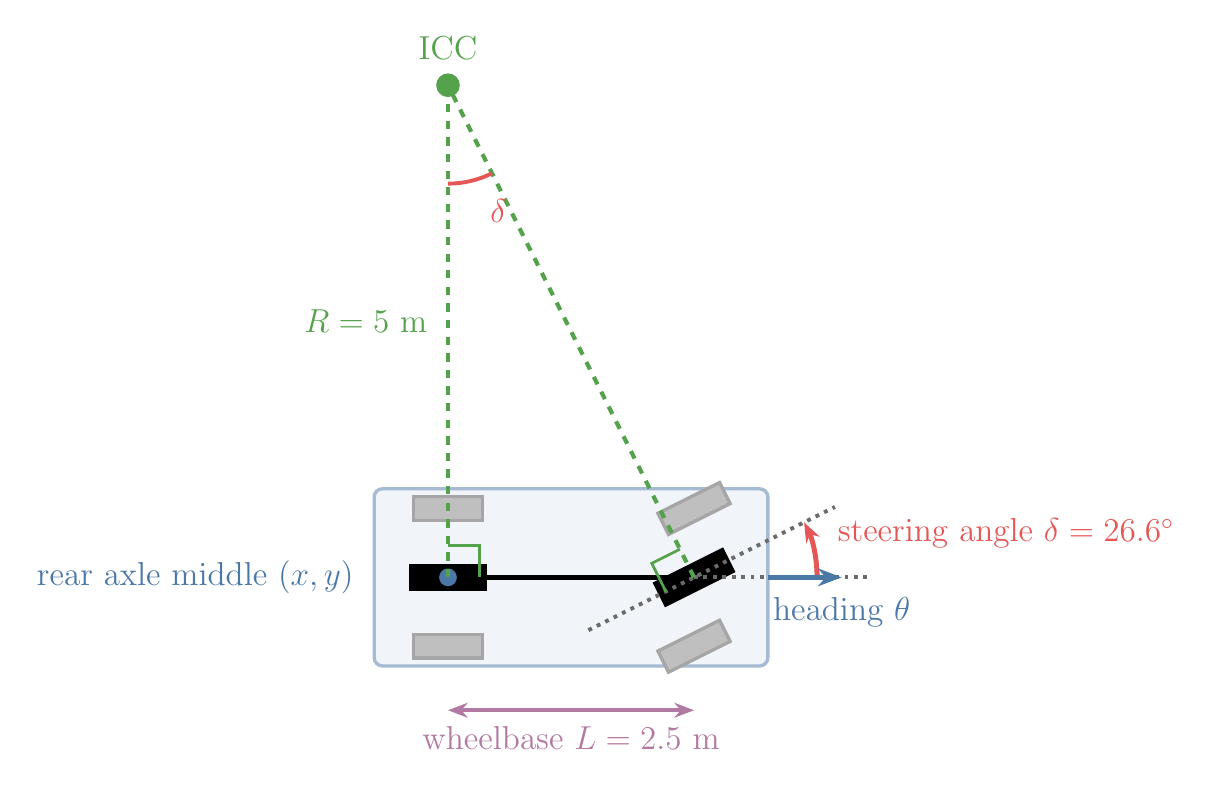
\begin{tikzpicture}[scale=1.25, every node/.append style={font=\large}]
  % car body (faint): 4.0 m x 1.8 m, rear axle 0.75 m from the rear bumper
  \draw[cblue!50, fill=cblue!8, rounded corners=3pt] (-0.75,-0.9) rectangle (3.25,0.9);
  % the four real wheels, faint
  \foreach \y in {0.7,-0.7} {
    \draw[black!35, fill=black!25] (-0.35,\y-0.12) rectangle (0.35,\y+0.12);
    \begin{scope}[shift={(2.5,\y)}, rotate=26.57]
      \draw[black!35, fill=black!25] (-0.35,-0.12) rectangle (0.35,0.12);
    \end{scope}
  }
  % bicycle: one rear wheel, one front wheel on the centre line
  \draw[line width=2pt] (0,0) -- (2.5,0);
  \fill[black] (-0.4,-0.14) rectangle (0.4,0.14);
  \begin{scope}[shift={(2.5,0)}, rotate=26.57]
    \fill[black] (-0.4,-0.14) rectangle (0.4,0.14);
    \draw[cgrey, dotted, line width=1.4pt] (-1.2,0) -- (1.6,0);
  \end{scope}
  \draw[cgrey, dotted, line width=1.4pt] (2.5,0) -- (4.3,0);
  % steering angle
  \draw[-{Stealth[length=2.5mm]}, cred, line width=1.8pt] (3.75,0) arc (0:26.57:1.25);
  \node[cred, anchor=west] at (3.85,0.45) {steering angle $\delta = 26.6^\circ$};
  % wheelbase
  \draw[{Stealth[length=2.5mm]}-{Stealth[length=2.5mm]}, cpurple, line width=1.5pt] (0,-1.35) -- (2.5,-1.35);
  \node[cpurple, below] at (1.25,-1.4) {wheelbase $L = 2.5$ m};
  % rear axle middle (the car's pose point)
  \fill[cblue] (0,0) circle (0.09);
  \node[cblue, anchor=east] at (-0.85,0) {rear axle middle $(x, y)$};
  % ICC and the two radii
  \fill[cgreen] (0,5) circle (0.12);
  \node[cgreen, anchor=south] at (0,5.15) {ICC};
  \draw[cgreen, dashed, line width=1.5pt] (0,0) -- (0,5);
  \draw[cgreen, dashed, line width=1.5pt] (2.5,0) -- (0,5);
  \node[cgreen, anchor=east] at (-0.1,2.6) {$R = 5$ m};
  % right angle marks
  \draw[cgreen, line width=1pt] (0,0.32) -- (0.32,0.32) -- (0.32,0);
  \begin{scope}[shift={(2.5,0)}, rotate=26.57]
    \draw[cgreen, line width=1pt] (0,0.32) -- (-0.32,0.32) -- (-0.32,0);
  \end{scope}
  % angle delta also at the ICC
  \draw[cred, line width=1.4pt] (0,4.0) arc (-90:-63.43:1.0);
  \node[cred, anchor=west] at (0.32,3.72) {$\delta$};
  % heading arrow
  \draw[-{Stealth[length=3mm]}, cblue, line width=2pt] (3.25,0) -- (4.0,0) node[pos=1.0, below=3pt] {heading $\theta$};
\end{tikzpicture}
\end{document}
